\section{Electronics and readout}

\F{electronicScheme} shows a schematic diagram of the electronics and readout used for the LTCC detector.

The XP4500B Photonis PMTs are powered with positive polarity by a CAEN SY4527 high voltage mainframe outfitted with 1501P boards.

There are two anode signals from the PMT output. One of them is connected directly to flash ADC
boards built at Jefferson Lab, the Flash ADC module FADC250\cite{daq2019}. The FADC250 sampling frequency is 250 $MHz$.
The other signal is discriminated by the Jefferson Lab built discriminator scaler module DSC2\cite{daq2019}, and connected to CAEN v1190 TDC modules.
The TDCs were set to have 50 ps/channel timing resolution, and the threshold was set to 30 mV, corresponding to 15\% of the SPE amplituted.

The LTCC FADC250 and TDC information are read out using the CLAS12 Data Acquisition system \cite{daq2019}.

\begin{figure}
	\centering
	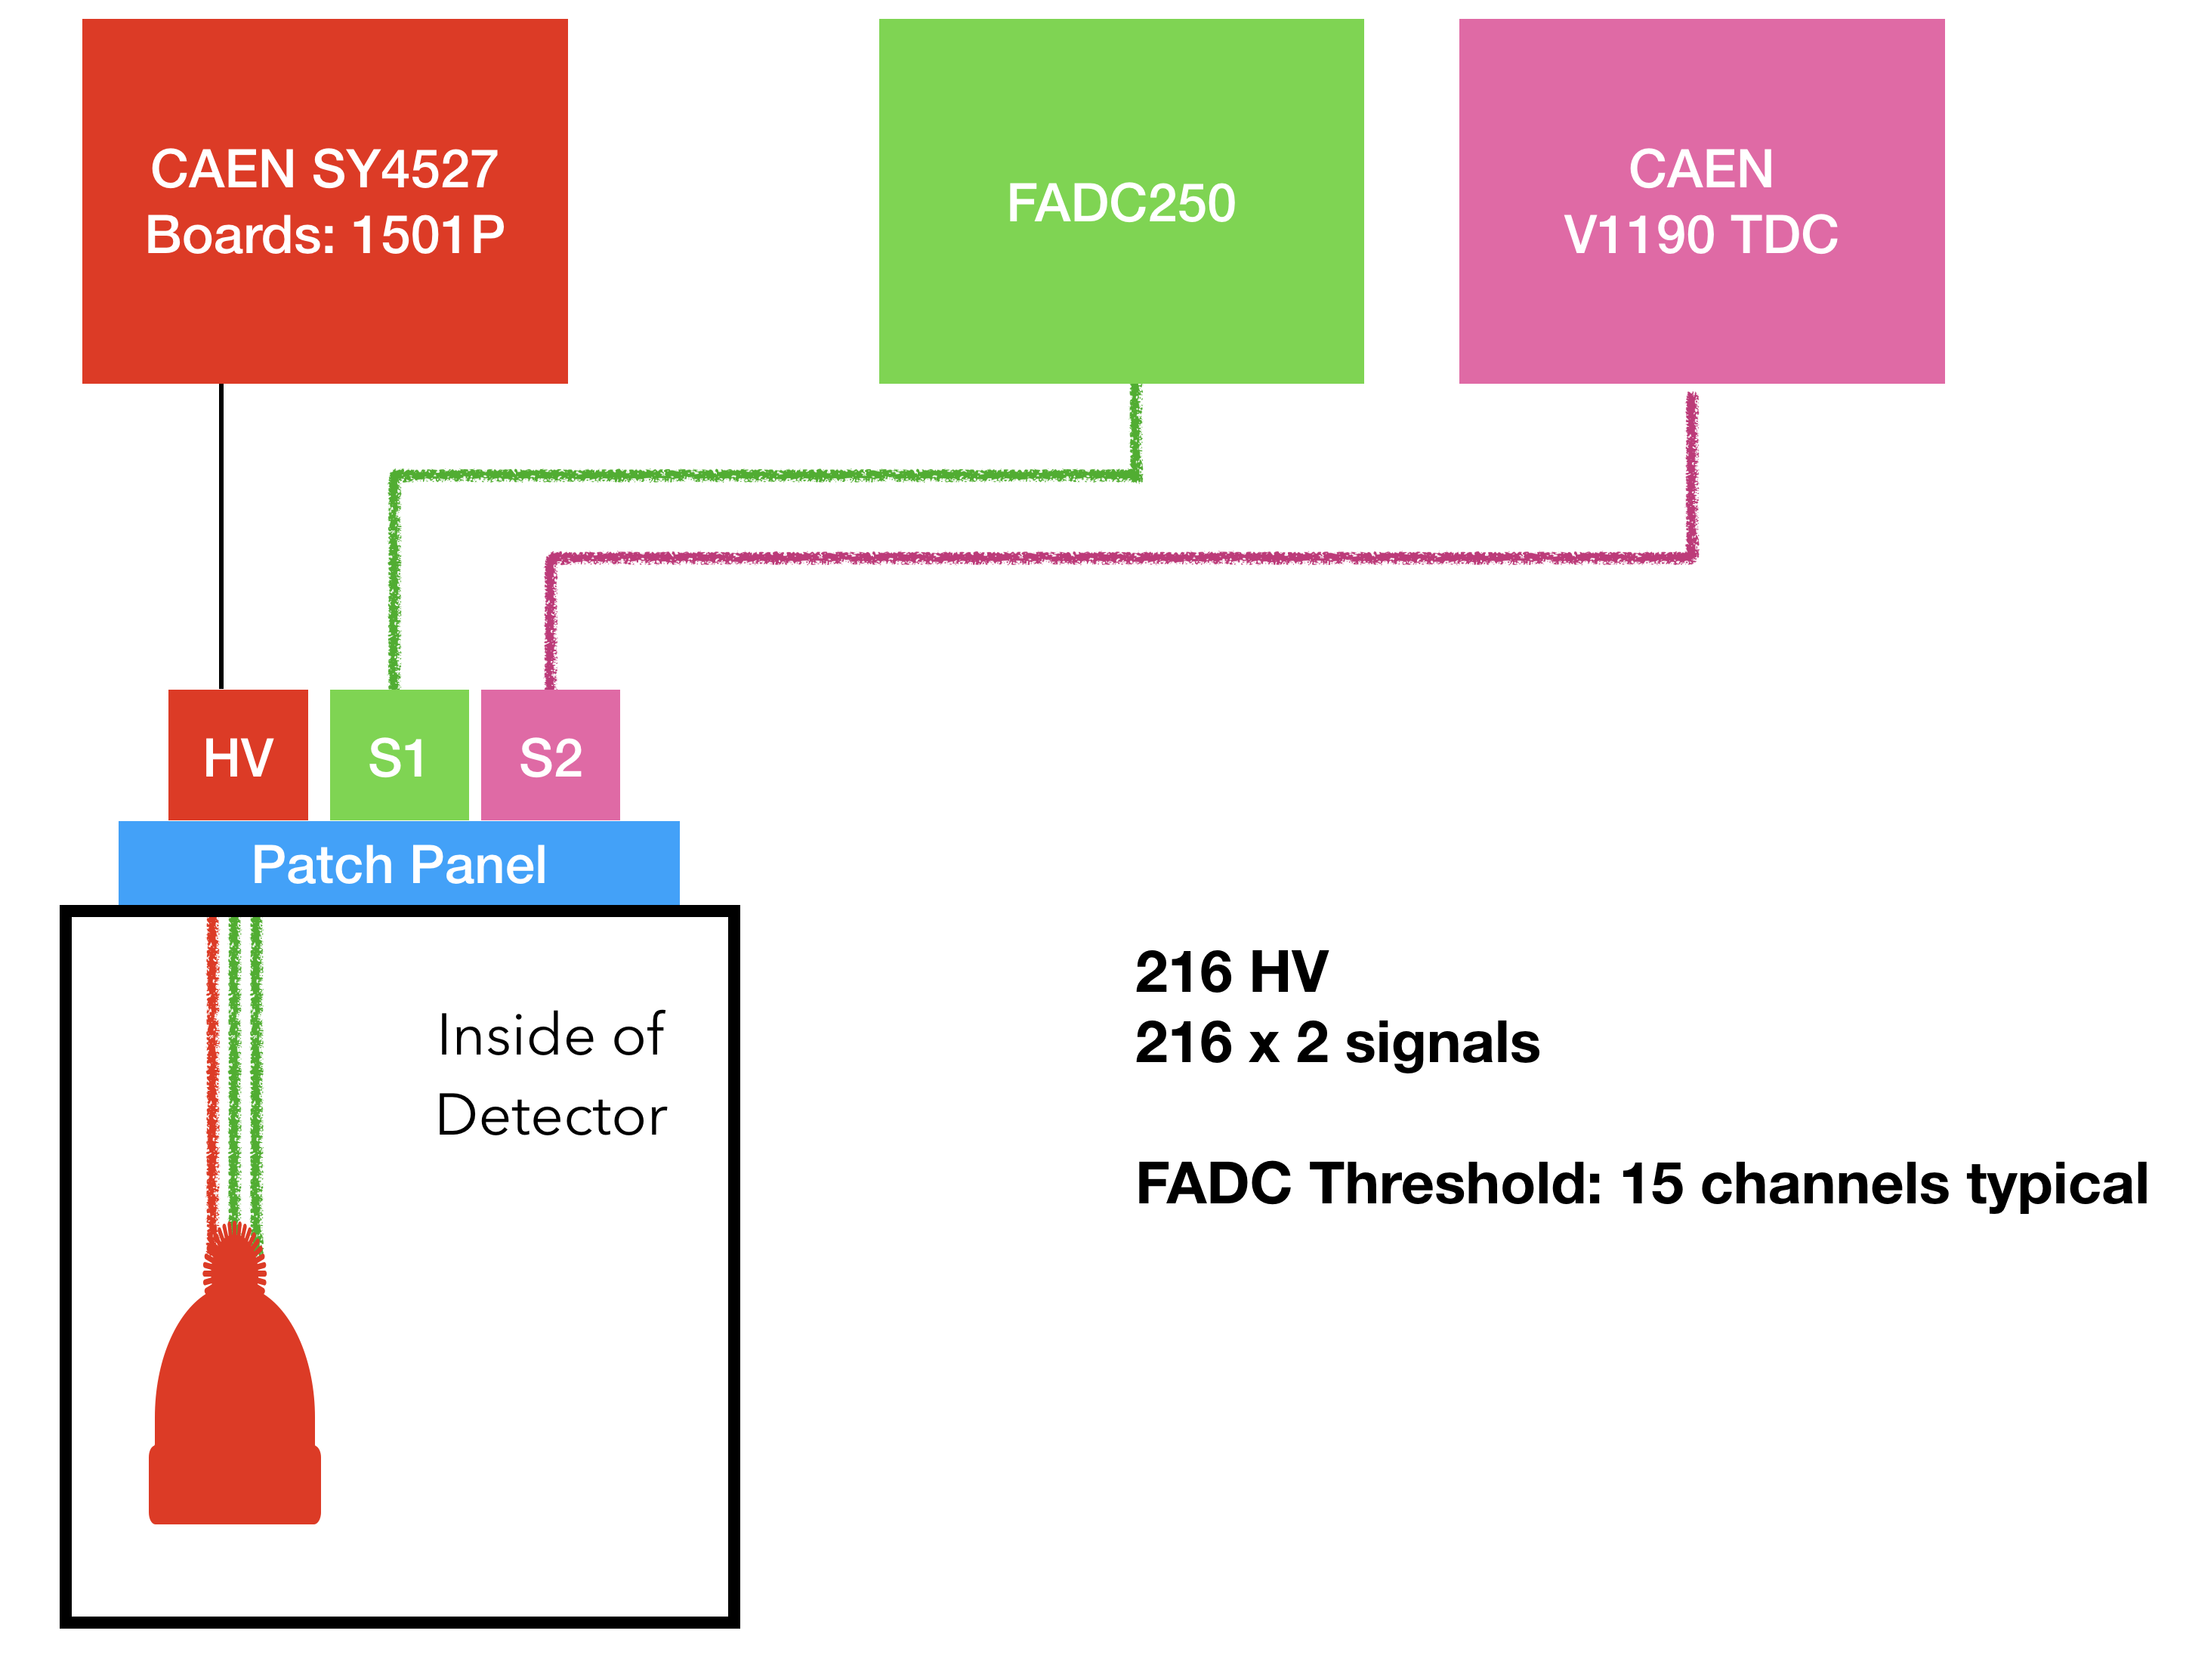
\includegraphics[width=0.99\columnwidth,keepaspectratio]{img/electronicScheme.png}
	\caption{The electronics schematic of the LTCC. One HV and two readout signals are connected from each PMT base to the patch panel.
		     The patch panels then connect the HV to the CAEN SY4527 (1501P boards), one readout to the FADC250
             and the other to DSC2 discriminators.}
	\label{fig:electronicScheme}
\end{figure}


A typical signal from the FADC250 module is shown in \F{fadc}. The signal is usually contained in 3 to 5 time samples
(each time sample is 4 ns).
In order to be written to tape, at least one of the 100 signals must be above a threshold of 30 channels, corresponding to about
30\% of the SPE peak value. This is well above the typical pedestal variation of 1-5 channels.
The FADC250 then considers a time window of 16 ns (4 samples) before the threshold crossing time, for the duration
of 20 samples (80 ns). The final integrated charge used in the reconstruction code is the signal integral
minus the electronic pedestal, as described in \F{fadc}.



\begin{figure}
	\centering
	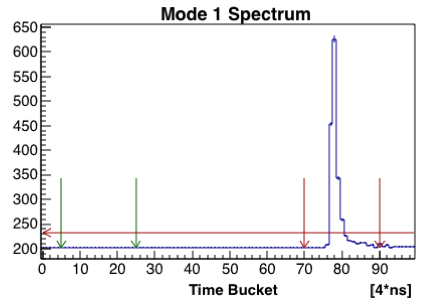
\includegraphics[width=0.99\columnwidth,keepaspectratio]{img/fadc.png}
	\caption{The FADC250 digitized output as a function of sample index of one of the LTCC PMTs.
             The DAQ system saves a 400 ns time window (100 samples) if at least one of the 100 signals is above a 30-channel threshold.
		     The integral signal is the sum of the output at the sample indexes between the two right arrows,
             one placed 4 samples before the signal crosses the threshold, and the other placed 20 samples after that.
             The final integrated charge used in the reconstruction code is this integral minus the pedestal.
             The pedestal is calculated using the average of the signal between the left arrows.
		     The absolute positions of the pedestal acquisition limits and the relative position of the signal integration
             limits are adjusted in the DAQ parameters and loaded before each run.}
	\label{fig:fadc}
\end{figure}




%\begin{figure}
%	\centering
%	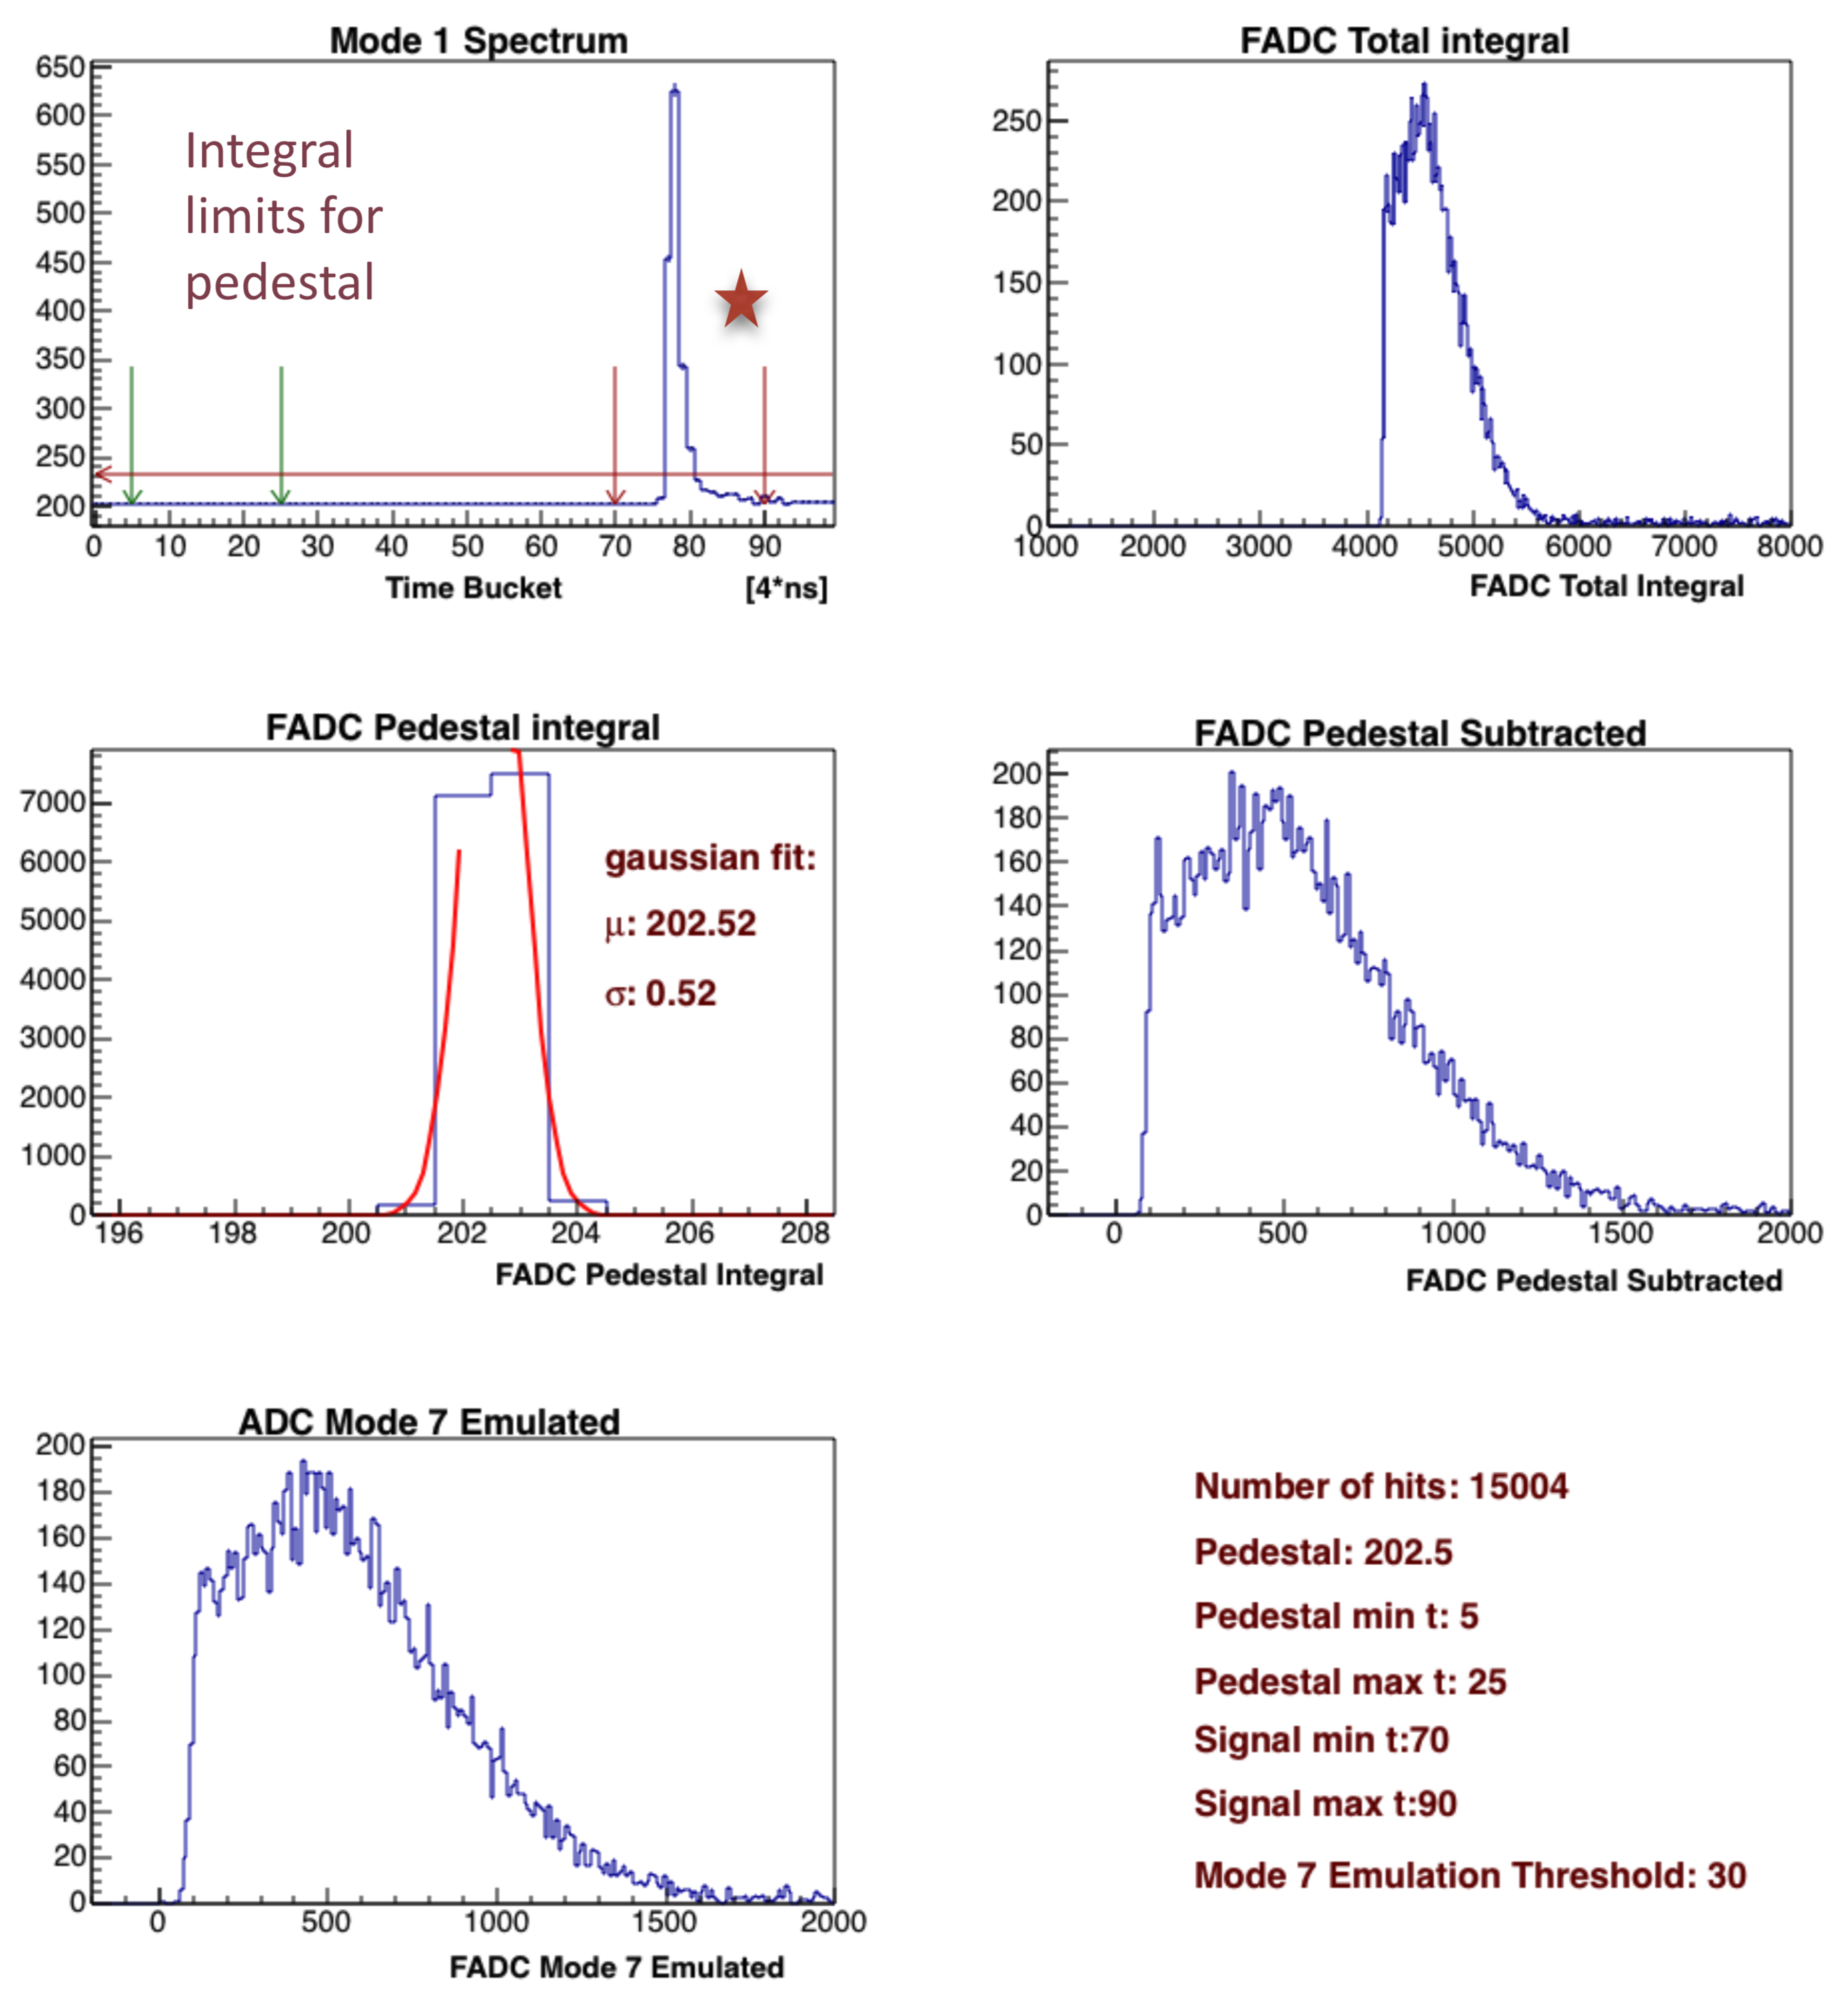
\includegraphics[width=0.99\columnwidth,keepaspectratio]{img/readout.png}
%	\caption{The electronic scheme of the LTCC.}
%	\label{fig:readout}
%\end{figure}
